% !TeX root = skripta-konstitutivni-vztahy.tex
% !TeX lastmodified = 2018-11-07

\subsection{Co je to predikční schopnost?}
Nejsou-li k~dispozici všechny potřebné mechanické zkoušky při různých typech napjatosti, je model nedostatečně experimentálně podložen.
Nejčastěji jsou konstanty modelu určeny jen z~jednoosé tahové zkoušky a~model musí predikovat (předpovědět) chování materiálu při jiném (víceosém) typu napjatosti. Přesnost, s~jakou to model dokáže, se nazývá jeho predikční schopností.

Odhad polohy deformačně-napěťových křivek ve dvouosé napjatosti vůči křivce určené z~jednoosé tahové zkoušky je možno udělat pro malé deformace z~Hookova zákona
\begin{equation}
	\sigma_1 = 2 G \varepsilon_1 + \lambda e = 2 G \varepsilon_1 + \lambda \left( \varepsilon_1 + \varepsilon_2 + \varepsilon_3 \right)
\end{equation}

Při tahovém zatížení ve směru 1 je tedy tuhost v~tomto směru při rovinné deformaci ($\varepsilon_2 = 0$) vždy větší než při jednoosé napjatosti (zde je $\varepsilon_2$ záporné a~tuhost odpovídá modulu pružnosti $E = \frac{\sigma_1}{\varepsilon_1}$). 
Při dvouosé napjatosti ($\varepsilon_2$ kladné) pak je tuhost ještě vyšší.
Pouze pro úplnou nestlačitelnost materiálu ($e = 0$) jsou odezvy při všech uvedených zkouškách (v~oblasti malých přetvoření) stejné.

Odezva izotropního materiálu při dvouosé napjatosti tedy není nikdy poddajnější než při jednoosé napjatosti.
Na druhé straně také nebývá mnohonásobně tužší.

\subsubsection{Predikční schopnost modelu Arruda-Boyce}
\begin{figure}[H]
	\centering
	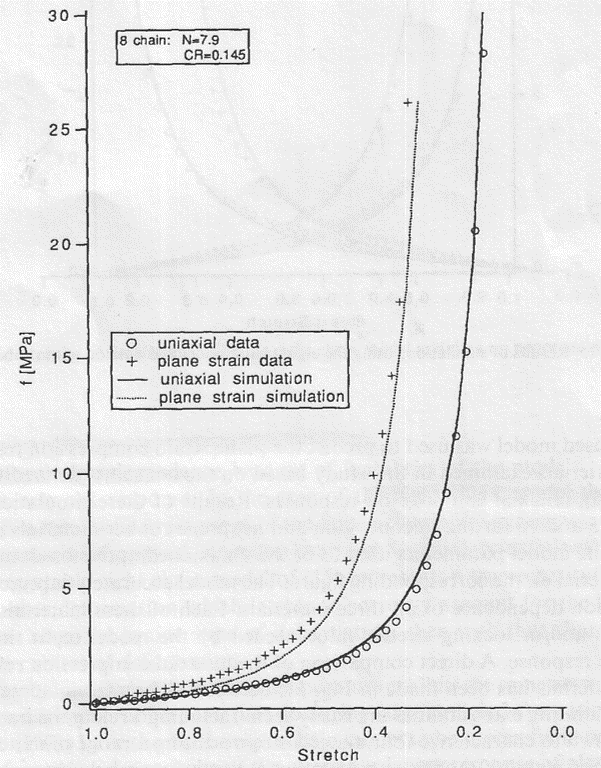
\includegraphics[height=5cm]{konstanty-tlak-arruda-boyce}
	\caption{Konstanty modelu určeny pouze z jednoosé tlakové zkoušky}
	\label{fig:konstanty-tlak-arruda-boyce}
\end{figure}
\begin{figure}[H]
	\centering
	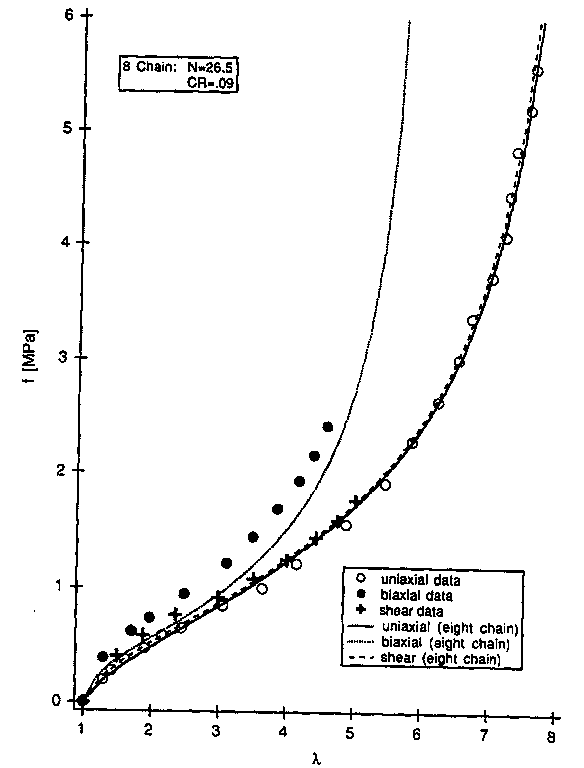
\includegraphics[height=5cm]{konstanty-tah-arruda-boyce}
	\caption{Konstanty modelu určeny pouze z jednoosé tahové zkoušky}
	\label{fig:konstanty-tah-arruda-boyce}
\end{figure}